\documentclass[24pt, a0papper, portrait]{tikzposter}
\makeatletter
\def\title#1{\gdef\@title{\scalebox{\TP@titletextscale}{%
\begin{minipage}[t]{\linewidth}
\centering
#1
\par
\vspace{0.5em}
\end{minipage}%
}}}
\makeatother
\usepackage[utf8]{inputenc}
\usepackage{subfig}
\usepackage{hyperref}
\hypersetup{
    colorlinks=true,
    urlcolor=blue,
    citecolor=black,
    linkcolor=black
}
\usepackage[retainorgcmds]{IEEEtrantools}
\graphicspath{ {./images/} }
 
\title{Simulation of Various Channelizer Structures 
       Directed by Cyclostationary Detector}
\author{Brian H. Hulette, Amir I. Zaghloul}
\institute{Virginia Tech Dept. of Electrical Engineering}
 
\usetheme{Autumn}
 
\begin{document}
 
\maketitle

\begin{columns}
\column{0.33}
\block{Introduction}
{
We present a Software-Defined Radio (SDR) system for detecting and tuning 
multiple signals of interest. 
Detection is performed by a cyclostationary detector, which
exploits the cyclostationary properties exhibited by most digital signals with
a fixed symbol rate.  Tuning, filtering, and decimating are performed by
a configurable filter bank, so that many signals can be isolated
simultaneously.  The block diagram shown in Figure~\ref{fig:block_diagram} 
illustrates this system.


%The system will sample
%at a high rate to acquire a large section of the frequency spectrum. Then it will attempt to
%detect the frequencies within the acquired range that contain signals of
%interest, and then tune, filter, decimate, and demodulate those signals. 

        \begin{tikzfigure}[High-level block diagram of our system. An analog front-end and
        ADC are used to bring wideband data into our Software-Defined Radio.
        There, a detector directs a configurable filter bank to isolate $N$
        signals of interest, which are then demodulated. The highlighted
        detector and filter bank are the components examined here.]
            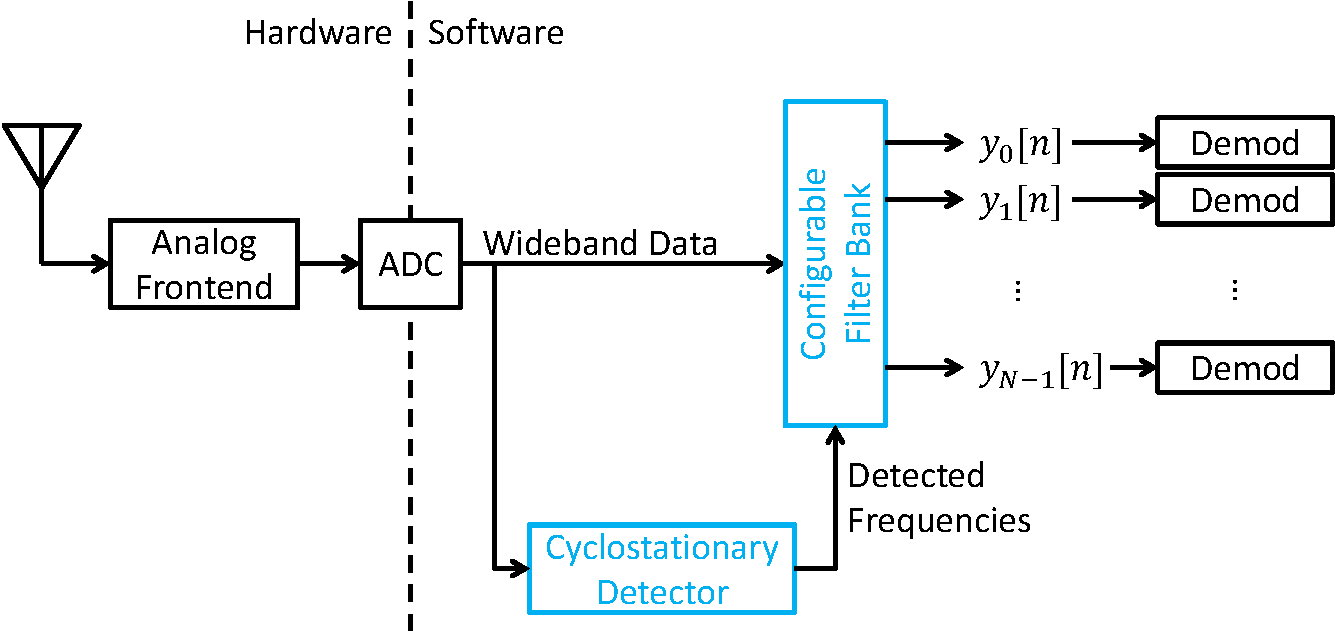
\includegraphics[width=0.9\linewidth]{block_diagram}
            \label{fig:block_diagram}
        \end{tikzfigure}

We are primarily concerned with two components: the cyclostationary detector,
and the configurable filter bank.  Two different filter bank structures are
examined: an overlap-save filter bank, and a combined polyphase
analysis/synthesis filter bank, composed of a polyphase analysis filter bank
followed by several polyphase synthesis filter banks.  These structures are
evaluated on two important criteria:
1) Their ability to accurately reproduce every detected signal, and 2) Their
   computational efficiency when combined with a cyclostationary detector.

    }
 
    \block{Cyclostationary Detection}
    {
Many digital communications exhibit a statistical property called
\emph{cyclostationarity}, which implies the signal has some parameter which
varies periodically with time. The frequency of this variation is called the cyclic
frequency, $\alpha$ \cite{Gardner1}. Of particular interest for us is second-order cyclostationarity,
where a signal has a periodic auto-correlation, $R_{xx}(t, t+\tau)$:

%\vspace{1cm}
\begin{IEEEeqnarray*}{lCl}
    R_{xx}(t, t+\tau) = E\{x(t)x^*(t+\tau)\} = \sum_{\alpha} R_{xx}^{\alpha}(\tau)e^{j2 \pi \alpha t}
\end{IEEEeqnarray*}
%\vspace{1cm}

The function $R_{xx}^{\alpha}(\tau)$ is the cyclic auto-correlation function (CAF), given by:

\begin{IEEEeqnarray*}{lCl}
    R_{xx}^{\alpha}(\tau) = \lim_{T \to \infty} \frac{1}{T}\int_{-T/2}^{T/2} R_{xx}(t, t+\tau)e^{-j2\pi \alpha t} dt
\end{IEEEeqnarray*}

Estimates of the CAF can be used for signal detection in the time
domain \cite{Jiandong1, Thai1, Oner1}. Another useful function for detection is the Fourier transform of the
CAF, called the Spectral Correlation Density (SCD), given by:

\begin{IEEEeqnarray*}{lCl}
    S_{xx}(\alpha, f) = \int_{-\infty}^{\infty} R_{xx}^{\alpha}(\tau)e^{-j2\pi f \tau} d\tau
\end{IEEEeqnarray*}

Estimates of the SCD can be used for detection in the frequency domain \cite{Oner1, Gardner2, Yoo1}, as illustrated in Figure~\ref{fig:scd}. This is the approach we use in our simulation.
        \begin{tikzfigure}[SCD Estimates for three QPSK signals at 156.25, 312.5, and 625 kbaud. SCD at $\alpha = 0$ Hz is equivalent to PSD, SCD at $\alpha=625$ Hz highlights signal at that baud rate.]
        \begin{minipage}[b]{0.45\linewidth}
            \centering
            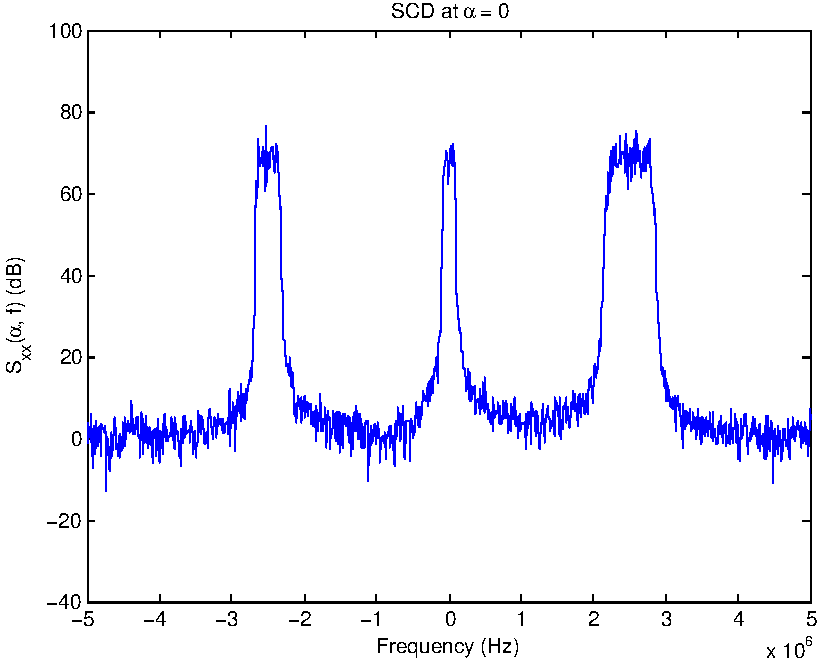
\includegraphics[width=\textwidth]{cyclo_0}
        \end{minipage}
        %\hspace{0.5cm}
        %\begin{minipage}[b]{0.45\linewidth}
        %    \centering
        %    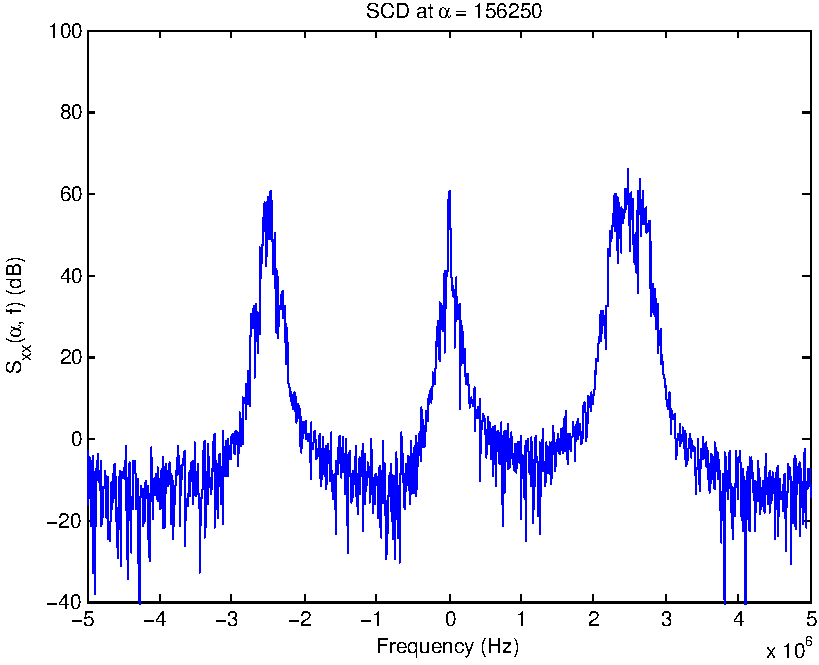
\includegraphics[width=\textwidth]{cyclo_156250}
        %    \label{fig:figure2}
        %\end{minipage}
        %\begin{minipage}[b]{0.45\linewidth}
        %    \centering
        %    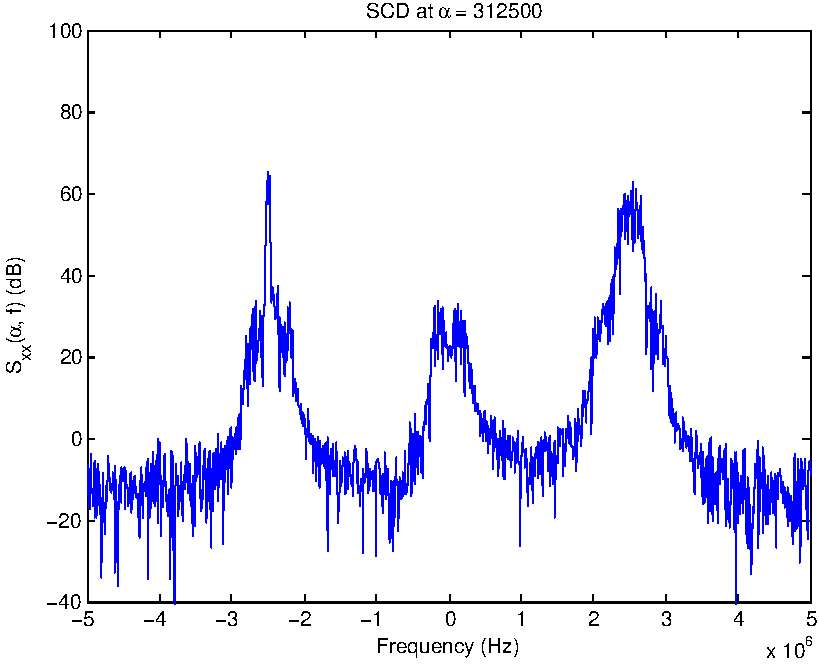
\includegraphics[width=\textwidth]{cyclo_312500}
        %    \label{fig:figure1}
        %\end{minipage}
        \hspace{0.5cm}
        \begin{minipage}[b]{0.45\linewidth}
            \centering
            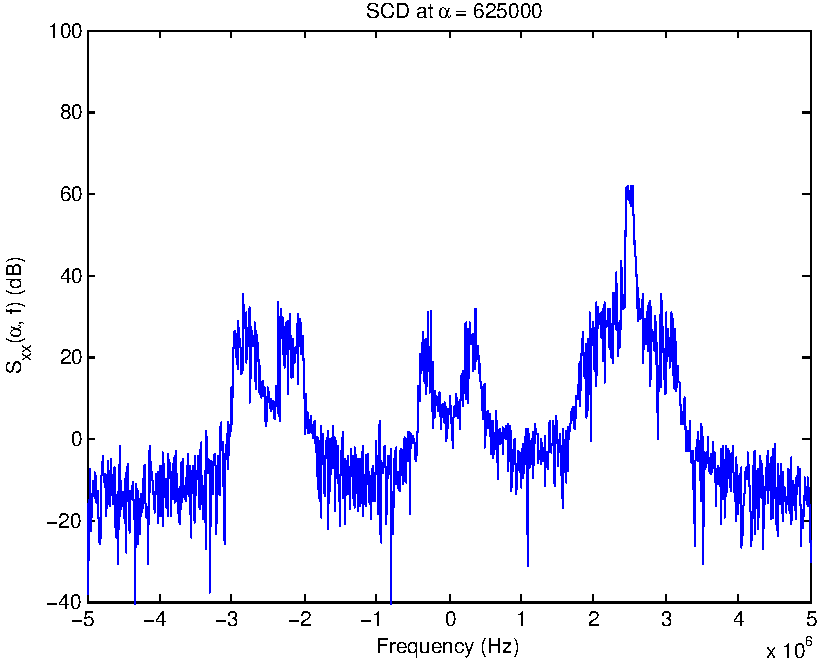
\includegraphics[width=\textwidth]{cyclo_625000}
        \end{minipage}
        \label{fig:scd}
        \end{tikzfigure}
    }
    \column{0.33}
    \block{Polyphase Filter Bank}
    {
        Polyphase analysis channelizers split a signal into $M$ channels separated in frequency by $f_s/M$ and decimated from the original sample rate by $D=M$. While synthesis channelizers perform the reverse process - combine $M$ channels \cite{Harris1}. Non-maximally decimated versions of these structures, where $D=M/2$ \cite{Chen1}, are shown in Figure \ref{fig:polyphase_structures}.

        \begin{center}
        \begin{tikzfigure*}
            \centering
            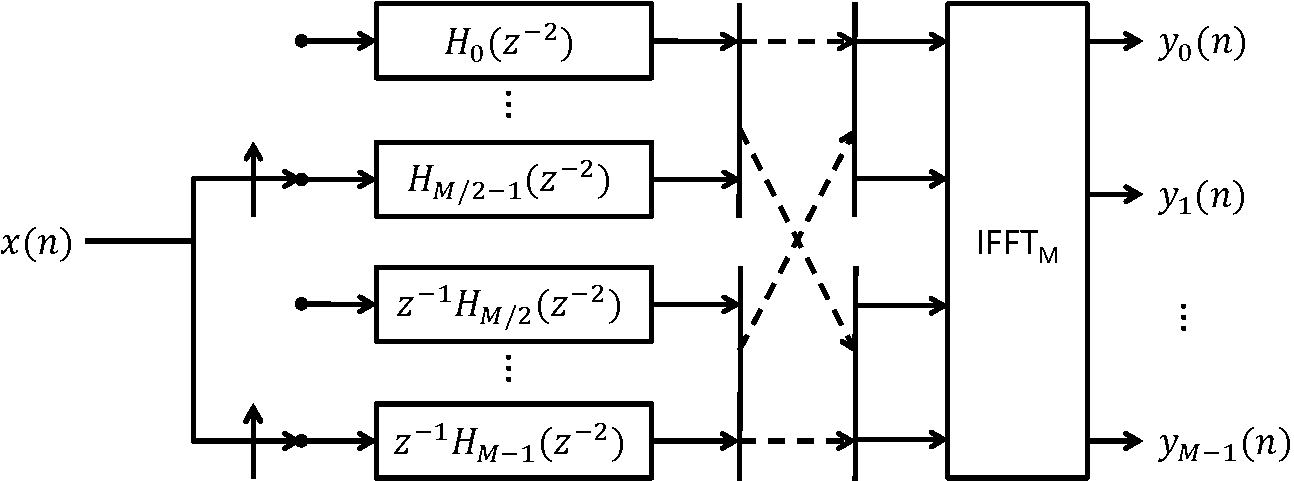
\includegraphics[width=0.65\linewidth]{polyphase_analysis_nmdfb}
        \end{tikzfigure*}
        \end{center}
        \begin{tikzfigure}[Non-maximally decimated ($D=M/2$) polyphase analysis and synthesis channelizers]
            \centering
            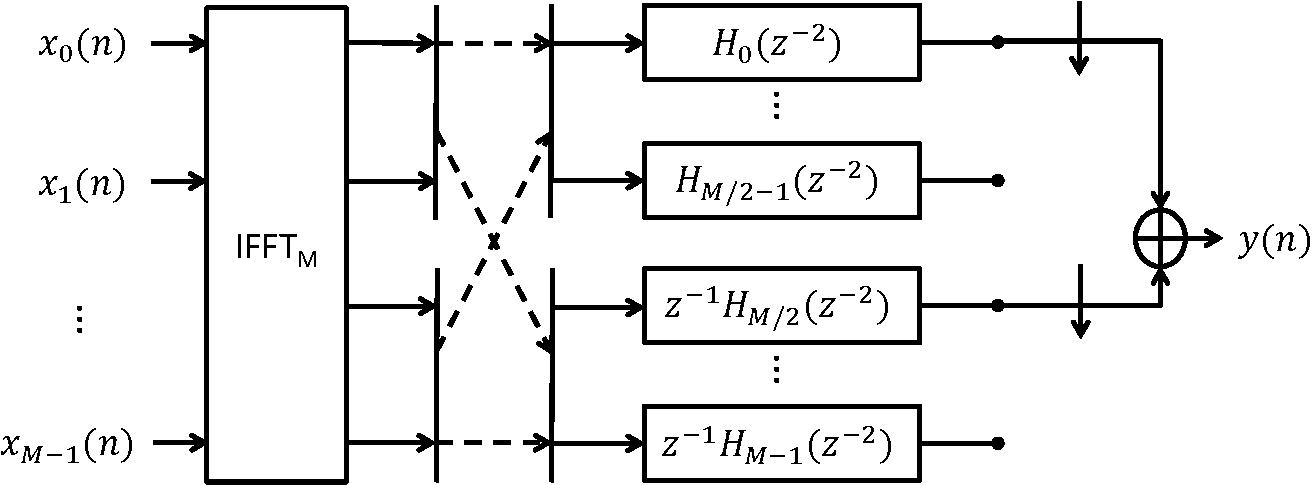
\includegraphics[width=0.65\linewidth]{polyphase_synthesis_nmdfb}
        \label{fig:polyphase_structures}
        \end{tikzfigure}
        Non-maximally decimated analysis and synthesis channelizers can be used
        together to first split up a frequency spectrum into several small,
        discrete channels, and reconstruct it around certain signals of
        interest \cite{Harris2}. This structure is shown in Figure
        \ref{fig:polyphase}.

        \begin{tikzfigure}[Using polyphase analysis and synthesis channelizers together to create a highly configurable and efficient filter bank. Note polyphase channelizers operate in the time domain, but in this figure signals are shown in the frequency domain to illustrate the concept.]
            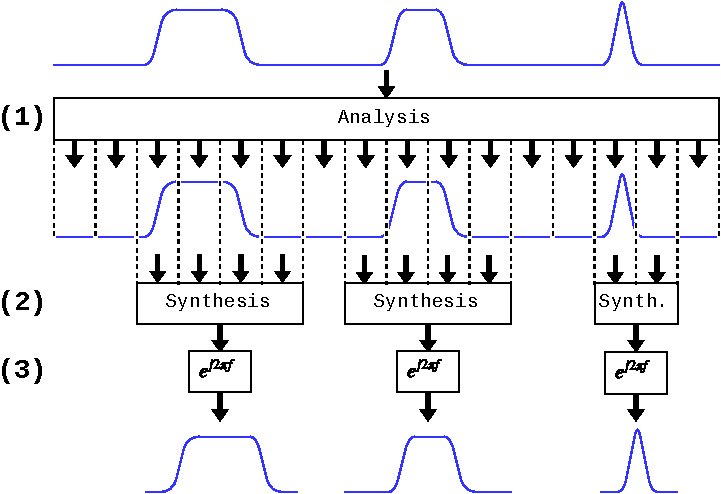
\includegraphics[width=0.75\linewidth]{polyphase}
            \label{fig:polyphase}
        \end{tikzfigure}
    }
    \block{Overlap-Save Filter Bank}
    {
        The Overlap-Save (OS) Filter Bank uses OS Fast Convolution to
        simultaneously isolate $N$ signals. By performing tuning in the
        frequency domain, or after the IFFT in the time-domain, as shown here,
        a single forward FFT can be re-used for all $N$ channels. This forward
        FFT can also be re-used for cyclostationary detection in certain
        situations, making for a very efficient structure.
        \begin{tikzfigure}[Using polyphase analysis and synthesis channelizers together to create a highly configurable and efficient filter bank.]
            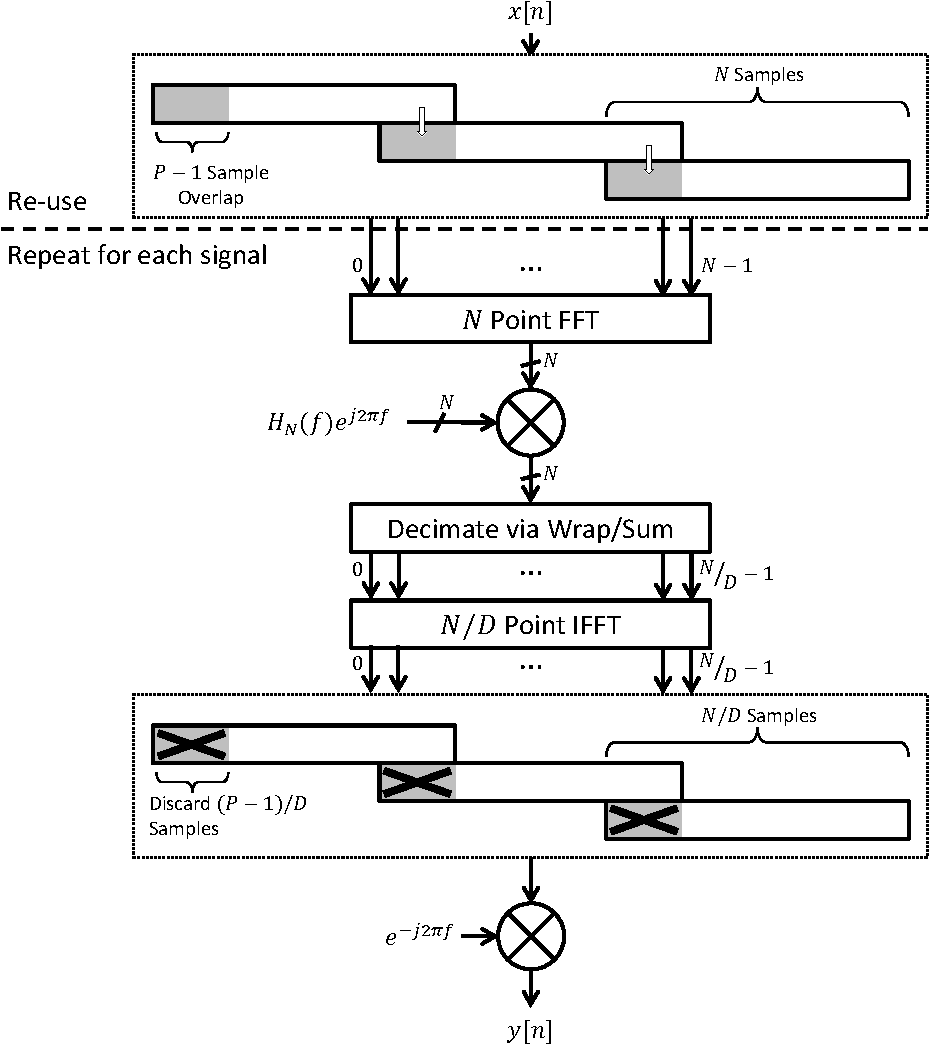
\includegraphics[width=0.85\linewidth]{overlap_save_time_domain}
        \end{tikzfigure}
        Decimation is also performed in the frequency domain via a ``wrap/sum" 
        approach, which means a smaller Inverse FFT can be used for each output \cite{Borgerding1}.
    }
    \column{0.33}
    \block{Simulation Results}
    {
A simulation of these structures has been created and used to compare the
efficiency of the two filter bank structures. A comparison of runtimes for the
overlap-save structure and the polyphase structure can be seen in
Figure~\ref{fig:runtime_comparison_250}. The plot shows the runtime when both
structures are used to simultaneously detect and tune various numbers of
signals. Each filter bank is configured to decimate every signal down to two
samples per symbol.

        \begin{tikzfigure}[Runtime comparison of detector combined with the overlap-save. Simulated 10 MHz acquisition with evenly spaced 78.125 ksymbol/s QPSK carriers.]
            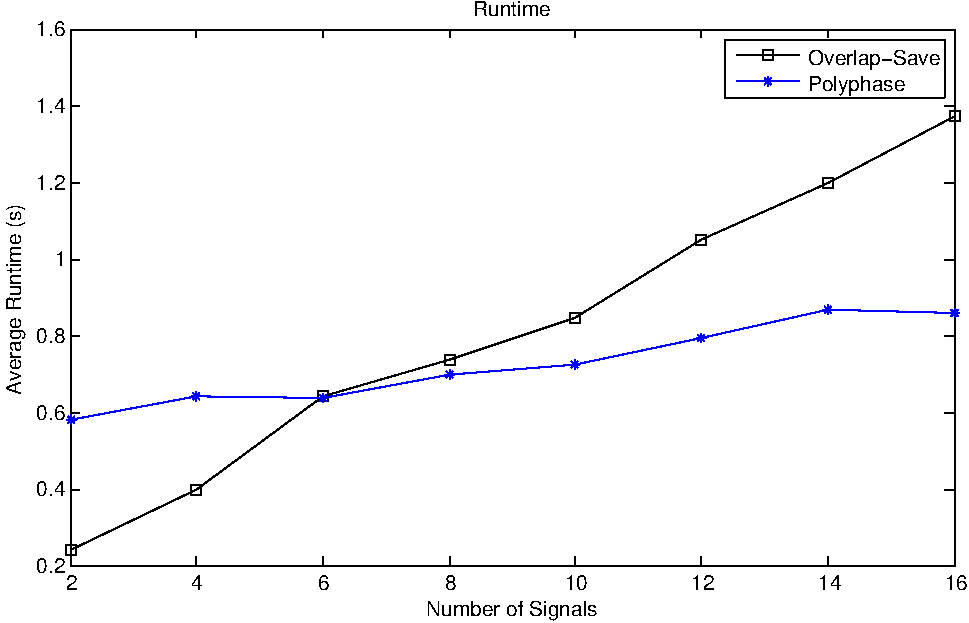
\includegraphics[width=0.8\linewidth]{runtime_comparison_250}
            \label{fig:runtime_comparison_250}
        \end{tikzfigure}

    
There are two clear takeaways from this result: 1) there is a larger up-front cost when using a polyphase filter bank, but 2) the
marginal cost for each additional signal being isolated is lower for the
polyphase filter bank. Thus for higher numbers of signals the polyphase filter bank can be more efficient.

\vspace{1cm}

The situation simulated in this scenario represents a best-case scenario for
both structures - the required decimation factor is a power of two. If a decimation
factor with a large prime factor is used then both channelizer structues must perform an inefficient FFT. Figure~\ref{fig:fft_runtime} illustrates this effect
for the polyphase filter bank.

\begin{tikzfigure}[Runtime comparison of detector combined with the polyphase filter
     bank. The 24.75248 kbaud signal requires a 202 point IFFT, while the 25
     kbaud signal can use a 200 point IFFT. The former has a large prime factor,
     101, leading to a much longer runtime. A similar effect can be seen in the
     overlap-save structure.]
    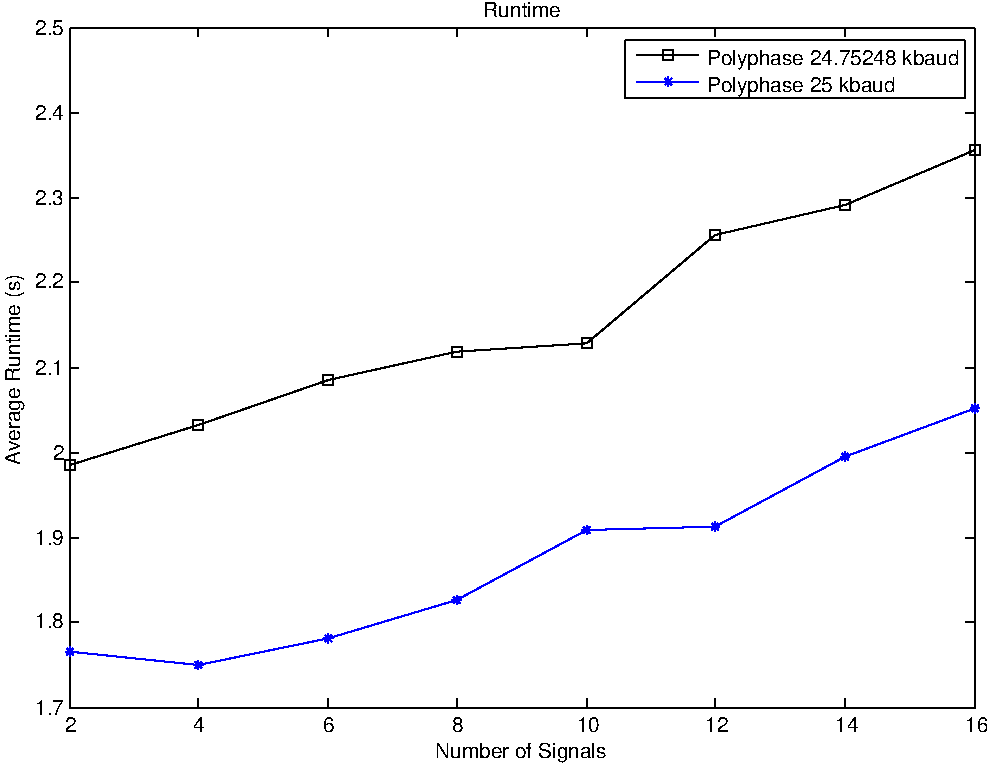
\includegraphics[width=0.8\linewidth]{fft_runtime_comparison}
    \label{fig:fft_runtime}
\end{tikzfigure}
    }

\block{References}
{
\footnotesize

\nocite{*}
\renewcommand\refname{}
\vspace*{-3cm}
\bibliographystyle{IEEEtran}
\bibliography{bibliography}
All of the source for this simulation is available on Github: \url{https://github.com/TheNeuralBit/cyclo_channelizer/}
}
\end{columns}

 
 
\end{document}
 
\end{document}
